\documentclass[12pt]{article}
\usepackage[top=1in, bottom=1in, left=1in, right=1in]{geometry}

\newif\ifeqns
\eqnstrue

\usepackage{setspace}
\onehalfspacing

\usepackage{amssymb}
%% The amsthm package provides extended theorem environments
\usepackage{amsthm}
\usepackage{epsfig}
\usepackage{times}
\renewcommand{\ttdefault}{cmtt}
\usepackage{amsmath}
\usepackage{graphicx} % for graphics files

% Draw figures yourself
\usepackage{tikz} 

% writing elements
\usepackage{mhchem}

% The float package HAS to load before hyperref
\usepackage{float} % for psuedocode formatting
\usepackage{xspace}

% from Denovo Methods Manual
\usepackage{mathrsfs}
\usepackage[mathcal]{euscript}
\usepackage{color}
\usepackage{array}

\usepackage[pdftex]{hyperref}
\usepackage[parfill]{parskip}

% math syntax
\newcommand{\nth}{n\ensuremath{^{\text{th}}} }
\newcommand{\ve}[1]{\ensuremath{\mathbf{#1}}}
\newcommand{\Macro}{\ensuremath{\Sigma}}
\newcommand{\rvec}{\ensuremath{\vec{r}}}
\newcommand{\omvec}{\ensuremath{\hat{\Omega}}}
%---------------------------------------------------------------------------
%---------------------------------------------------------------------------
\begin{document}
\begin{center}
{\bf NE 250, F17 \\
Fission\\
August 25, 2017}
\end{center}

\setlength{\unitlength}{1in}
\begin{picture}(6,.1) 
\put(0,0) {\line(1,0){6.25}}         
\end{picture}

%---------------------------------------------------------------------------
\section*{Fission}

The main goal of nuclear reactor theory is the utilization of the energy released by a controlled chain reaction of nuclear fission events. An example fission reaction:
 \[
 n+^{235}\text{U} \rightarrow \text{fission products + more neutrons +} \approx 200MeV
\]

The kinetic energy is then converted into heat as the released particles slow down by bouncing around in the reactor. (Note: 1eV = 1.602$\times 10^{-19}$J)

Just as important is the fact that the fission reaction produces a few neutrons that will induce other fission reactions, creating a chain reaction.

Fission is a threshold reaction; in the process of $^{236}$U splitting, there are several competing forces (Coulomb, nuclear).

$n+^{235}$U$\rightarrow ^{236}$U$^* \rightarrow A_1+A_2$, where $A_1 \approx A_2\approx$ half of 236

The stability of heavy nuclei against spontaneous fission is due to the potential energy barrier that must be overcome before the nucleus will fission. The size of this fission barrier is usually 6-9 MeV in most heavy nuclei of interest. The critical energy is the threshold necessary to be overcome in order for fission to occur.

The energy required to break down a nucleus into its component nucleons is called the nuclear binding energy. We frequently look at the binding energy per nucleon. The larger the binding energy per nucleon, the greater the work that must be done to remove the nucleon from the nucleus, the more stable the nucleus. Important features of the graph:
%https://www.miniphysics.com/binding-energy-per-nucleon-and-nuclear.html

\begin{itemize}
\item Excluding the lighter nuclei, the average binding energy per nucleon is about 8 MeV.
The maximum binding energy per nucleon occurs at around mass number A = 50, and corresponds to the most stable nuclei. Iron nucleus Fe-56 is located close to the peak with a binding energy per nucleon value of approximately 8.8 MeV. It's one of the most stable nuclides that exist.
\item Nuclei with very low or very high mass numbers have lesser binding energy per nucleon and are less stable because the lesser the binding energy per nucleon, the easier it is to separate the nucleus into its constituent nucleons.
\item Nuclei with low mass numbers may undergo nuclear fusion, where light nuclei are joined together under certain conditions so that the final product may have a greater binding energy per nucleon.
\item Nuclei with high mass numbers may undergo nuclear fission, where the nucleus split to give two daughter nuclei with the release of neutrons. The daughter nuclei will possess a greater binding energy per nucleon.
\end{itemize}


\begin{center}
\includegraphics[scale=0.6]{../figs/nucleonbinding}
\end{center}


\textit{Fissile isotopes} are those that can fission from a neutron with low (in theory, zero) kinetic energy: $^{233}$U, $^{235}$U, $^{239}$Pu, and $^{241}$Pu. [It is relevant to mention thermal neutrons, with very small kinetic energies.] Fissile nuclides represent the principle fuels used in fission chain-reaction systems. 

\textit{Fissionable isotopes} can undergo fission from high-energy neutrons; their critical energies are higher than those of fissile isotopes: $^{232}$Th, $^{238}$U, $^{240}$Pu. Fissionable nuclides are unable to sustain a stable fission reaction by themselves.

\textit{Fertile isotopes} are those that create fissile isotopes upon neutron capture. Two examples:
\ifeqns
$^{238}\text{U}+n \stackrel{\gamma}{\rightarrow} \, ^{239}\text{U}\stackrel{\beta^-}{\rightarrow} \, ^{239}\text{Np}\stackrel{\beta^-}{\rightarrow} \, ^{239}\text{Pu}$

$^{232}\text{Th}+n \stackrel{\gamma}{\rightarrow} \,^{233}\text{Th}\stackrel{\beta^-}{\rightarrow}\, ^{233}\text{Pa}\stackrel{\beta^-}{\rightarrow} \, ^{233}\text{U}$
\else
\vspace*{3 em}
\fi

Each fission of a parent atom produces a different set of fission product atoms, which also vary according to the energy of neutron inducing fission -- see \autoref{fig:fp-e} and \autoref{fig:fp-i}. However, while an individual fission is not predictable, the fission products are statistically predictable. The amount of any particular isotope produced per fission is called its yield, typically expressed as percent per parent fission.

\begin{figure}
\centering
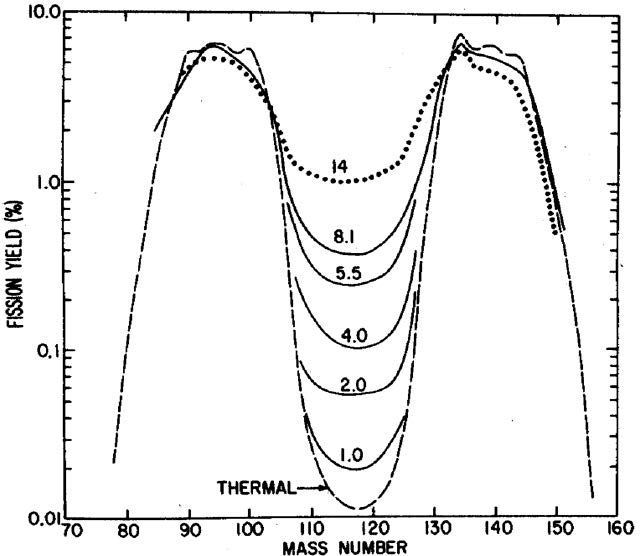
\includegraphics[scale=0.7]{../figs/FP_energy}
\caption{Fission product distribution from U-238 as a function of energy (MeV)}
\label{fig:fp-e}
\end{figure}
\begin{figure}
\centering
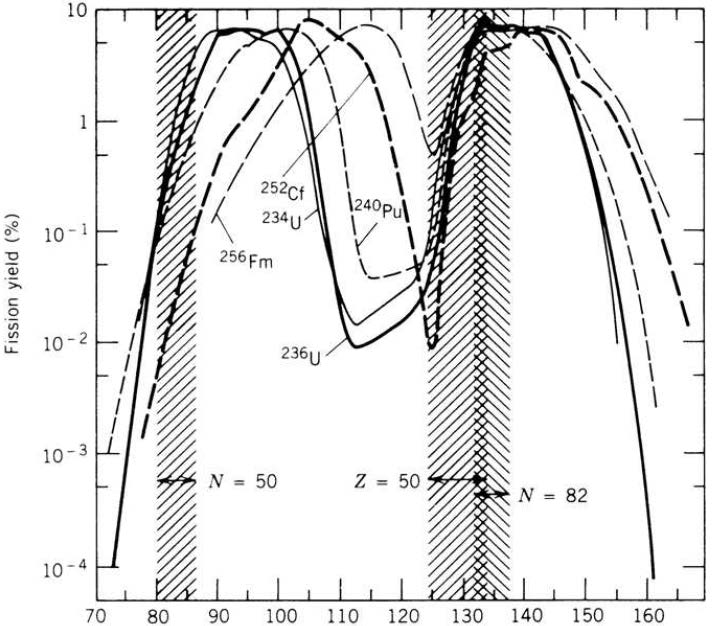
\includegraphics[scale=0.7]{../figs/FP_Isotope}
\caption{Fission product distribution from different isotopes}
\label{fig:fp-i}
\end{figure}

Most fission is asymmetric, with one fission product more massive than the other. In general, the higher the energy of the state that undergoes nuclear fission, the more likely that the two fission products have similar mass. Hence as the neutron energy increases and/or the energy of the fissile atom increases, the valley between the two peaks becomes more shallow.

We also care a lot about
$\nu$, the average number of neutrons per fission. See \autoref{fig:nu} for examples, where $\nu^{49}$ is for $^{239}$Pu, $\nu^{25}$ is for $^{235}$U, $\nu^{23}$ is for $^{233}$U.
\begin{figure}
\begin{center}
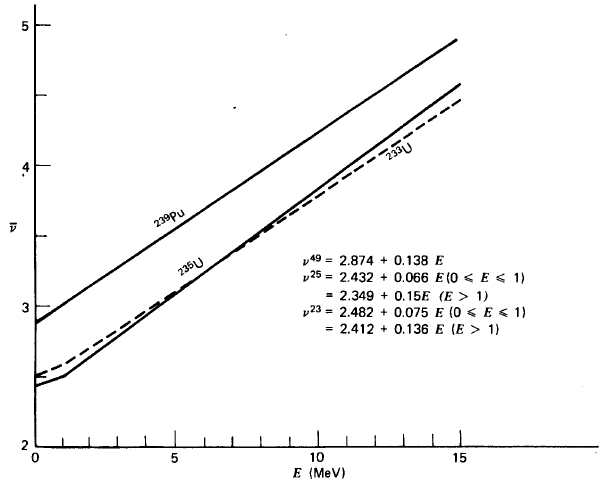
\includegraphics[scale=0.6]{../figs/nu}
\caption{average \# of neutrons released per fission as a function of energy}
\label{fig:nu}
\end{center}
\end{figure}


$\alpha = \frac{\sigma_\gamma}{\sigma_f}$ is the capture-to-fission ratio

$\eta = \frac{\nu \sigma_f}{\sigma_a}$ is the average number of neutrons produced per neutron absorbed. For a single fissile isotope we can write $\eta = \frac{\nu}{1+\alpha}$

conversion ratio = $\frac{\text{fissile produced}}{\text{fissile consumed}}$

In thermal reactors, the conversion ratio is typically less than one. In fast reactors, the conversion ratio can be greater than or equal to one. This is the motivation for ``breeding" reactors and requires $\eta >2$.

\begin{figure}
\begin{center}
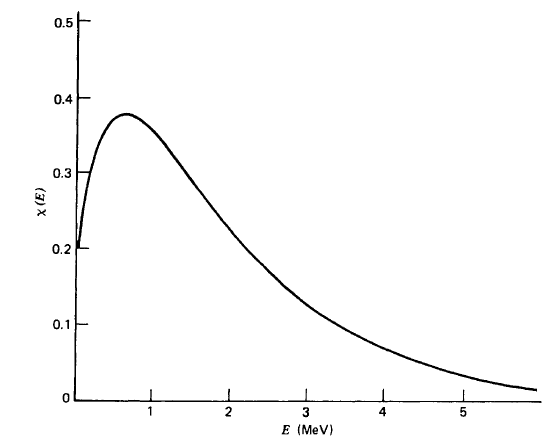
\includegraphics[scale=0.6]{../figs/fissionspectrum}
\caption{Fission spectrum for thermal neutron induced fission in $^235$U}
\label{fig:spectrum}
\end{center}
\end{figure}
%
$\chi(E)dE=$ fission spectrum = probability that a neutron will have energy\\ $E$ in the range $[E, E+dE]$ (see \autoref{fig:spectrum})

The prompt neutron fission spectrum of $^{235}$U: $\chi(E) = 0.453 e^{-1.036E}\sinh\sqrt{2.29E}$

Fission produces both prompt and delayed neutrons, where the delayed neutrons come from the decay of various unstable fission products. We define: $\beta=\frac{\nu_{delayed}}{\nu_{total}}$. Delayed neutrons are usually split into six groups, based on the half-lifes of the unstable fission products.

The majority of the energy released in a fission event is in form of the kinetic energy of the fission products. For $^{235}$U fission:

\ifeqns
KE of FP $\approx 168$ MeV

KE of $n\approx 5$ MeV

prompt $\gamma$ E$\approx 7$ MeV

$\beta^- $ E from FP decay $\approx 8$ MeV

$\gamma $ E from FP decay $\approx 7$ MeV

neutrino E from FP decay $\approx 12$ MeV
\else
\vspace*{6 em}
\fi

All of the kinetic energy from the fission products and neutrons is considered recoverable. Most of the $\gamma$ energy and all of the $\beta^-$ energy is recoverable. None of the neutrino energy is recoverable. In total, $~207$ MeV is emitted and $~195$MeV is recoverable.

\section*{Multiplication Factor and Nuclear Criticality}

$k=\frac{\text{\# of neutrons produced}}{\text{\# of neutrons lost}}$ (multiplication factor)

$p=$ resonance escape probability = fraction of fission neutrons that manage to slow down from fission to thermal energies without being absorbed.

$f=$ thermal utilization factor = conditional probability that if neutron is absorbed, it will be absorbed in the fuel.

$\epsilon=$ fast fission factor = total number of fission neutrons / number of fission neutrons from thermal fission.

The four-factor formula assumes an infinite homogeneous system with two neutron groups (fast + thermal):
\[
k_{\infty}=\epsilon p f \eta
\]

The six-factor formula accounts for fast and thermal neutron leakage in finite systems:
\[
k_{eff} = P_{FNL}P_{TNL}\epsilon p f\eta
\]

We determine the state of criticality using $k$, with $k=1$ being critical (sustaining reaction), $k<1$ subcrictical (decreasing), and $k>1$ supercritical (increasing). We'll talk more about this later in class.


\end{document}
